\documentclass[a4paper]{article}
\usepackage{import}
\usepackage[utf8]{inputenc}
\usepackage[T1]{fontenc}
\usepackage{textcomp}
\usepackage[italian]{babel}
\usepackage{amsmath, amssymb}
\usepackage{booktabs,xltabular}
\usepackage{amsfonts}
\usepackage{subcaption}
\usepackage{amsthm}
\usepackage{cancel}
\usepackage{mdframed}
\usepackage{makecell}
\usepackage{float}
\usepackage{xcolor}
\usepackage{listings}
\usepackage{gensymb}
\usepackage{graphicx}
\usepackage{bodeplot}
\usepackage{physics}
\usepackage{tikz}
\usetikzlibrary{shapes, arrows, automata, petri, decorations.markings, decorations.pathreplacing, positioning, calc, quotes}
\usepackage{circuitikz}
\usepackage[label=corner]{karnaugh-map}
\graphicspath{{./figures/}}

% Set default font to sans-serif
\renewcommand{\familydefault}{\sfdefault} 
\usepackage{eulervm}

\usepackage{forest}

\usepackage{mathtools}
\DeclarePairedDelimiter\ceil{\lceil}{\rceil}
\DeclarePairedDelimiter\floor{\lfloor}{\rfloor}

% \usepackage{ntheorem}

\usepackage{import}
\usepackage{pdfpages}
\usepackage{transparent}
\usepackage{xcolor}

\usepackage{hyperref}
\hypersetup{
    colorlinks=false,
}

% Code blocks
\definecolor{codegreen}{rgb}{0,0.6,0}
\definecolor{codegray}{rgb}{0.5,0.5,0.5}
\definecolor{codepurple}{rgb}{0.58,0,0.82}
\definecolor{backcolour}{rgb}{0.95,0.95,0.95}

\lstdefinestyle{mystyle}{
	backgroundcolor=\color{backcolour},
	commentstyle=\color{codegreen},
	keywordstyle=\color{magenta},
	numberstyle=\tiny\color{codegray},
	stringstyle=\color{codepurple},
	basicstyle=\ttfamily\footnotesize,
	breakatwhitespace=false,
	breaklines=true,
	captionpos=b,
	keepspaces=true,
	numbers=left,
	numbersep=5pt,
	showspaces=false,
	showstringspaces=false,
	showtabs=false,
	tabsize=2
}

\lstset{style=mystyle}

\usepackage{color}
\usepackage{import}
\usepackage{pdfpages}
\usepackage{transparent}
\usepackage{xcolor}

% Example frame
\theoremstyle{definition}
\newmdtheoremenv[%
	linecolor=gray,leftmargin=0,%
	rightmargin=0,
	innertopmargin=8pt,%
	innerbottommargin=8pt,
	ntheorem]{example}{Esempio}[section]

% Important definition frame
\theoremstyle{definition}
\newmdtheoremenv[%
	linecolor=gray,leftmargin=0,%
	rightmargin=0,
	backgroundcolor=gray!40,%
	innertopmargin=8pt,%
	innerbottommargin=8pt,
	ntheorem]{definition}{Definizione}[section]

% Exercise frame
\theoremstyle{definition}
\newmdtheoremenv[%
	linecolor=gray,leftmargin=0,%
	rightmargin=0,
	innertopmargin=8pt,%
	innerbottommargin=8pt,
	ntheorem]{exercise}{Esercizio}[section]

% Theorem frame
\theoremstyle{definition}
\newmdtheoremenv[%
  linecolor=gray,leftmargin=0,%
  rightmargin=0,
  innertopmargin=8pt,%
  innerbottommargin=8pt,
  ntheorem]{theorem}{Teorema}[section]

\theoremstyle{definition}
\newmdtheoremenv[%
  linecolor=white,leftmargin=0,%
  rightmargin=0,
  innertopmargin=8pt,%
  innerbottommargin=8pt,
  ntheorem]{define}{Definizione utile}[section]

% figure support
\usepackage{import}
\usepackage{xifthen}
\pdfminorversion=7
\usepackage{pdfpages}
\usepackage{transparent}
\newcommand{\incfig}[1]{%
	\def\svgwidth{\columnwidth}
	\import{./figures/}{#1.pdf_tex}
}

% FSM tikz
\tikzset{
    place/.style={
        circle,
        thick,
        draw=black,
        minimum size=6mm,
    },
        state/.style={
        circle,
        thick,
        draw=black,
        fill=white,
        minimum size=6mm,
    },
}

\pdfsuppresswarningpagegroup=1

\usepackage{pgfplots}
\pgfplotsset{compat=1.18,width=10cm}

% Save plots as pdf and reuse them without compiling every time
\usetikzlibrary{external}
\tikzexternalize[prefix=figures/tikz/, optimize=false]


\begin{document}

\begin{titlepage}
	\begin{center}
		\vspace*{1cm}

		\Huge
		\textbf{Probabilità e Statistica\\Esercizi}

		\vspace{0.5cm}
		\LARGE
		UniVR - Dipartimento di Informatica

		\vspace{1.5cm}

		\textbf{Fabio Irimie}

		\vfill


		\vspace{0.8cm}


		2° Semestre 2023/2024

	\end{center}
\end{titlepage}


\tableofcontents
\pagebreak

\section{Introduzione}
Il problema principale che bisogna affrontare è la comunicazione tra 2 calcolatori,
cioè lo scambio di informazioni. Per far comunicare 2 calcolatori c'è bisogno di
alcuni requisiti:
\begin{enumerate}
  \item \textbf{Protocollo}: È un insieme di regole che sovraintende alla comunicazione,
    in cui si definiscono:
    \begin{itemize}
      \item Il formato dei messaggi
      \item Le azioni da intraprendere nel gestire i messaggi stessi
    \end{itemize}
    Questo perchè per comunicare tutti devono "parlare la stessa lingua".

  \item \textbf{Architettura di rete}: Come, fisicamente, trasportare i messaggi
\end{enumerate}

\begin{figure}[H]
  \begin{example}
    Prendiamo ad esempio la scrittura e la spedizione delle lettere. Ci sono 2
    utenti che vogliono scambiare delle lettere.
    
    Per gestire il trasporto della
    lettera essa viene messa all'interno di una \textbf{busta}, che contiene informazioni
    su dove deve essere spedita. Una volta inbustata, va imbucata in una cassetta 
    delle lettere da cui poi verrà prelevata e mandata alla cassetta delle lettere 
    del secondo utente dalla \textbf{rete} di distribuzione degli uffici postali.

    L'utente poi preleverà la lettera dalla cassetta delle lettere e dopo aver
    controllato le informazioni sulla busta, la aprirà e leggerà il contenuto.
    \begin{figure}[H]
      \begin{center}
        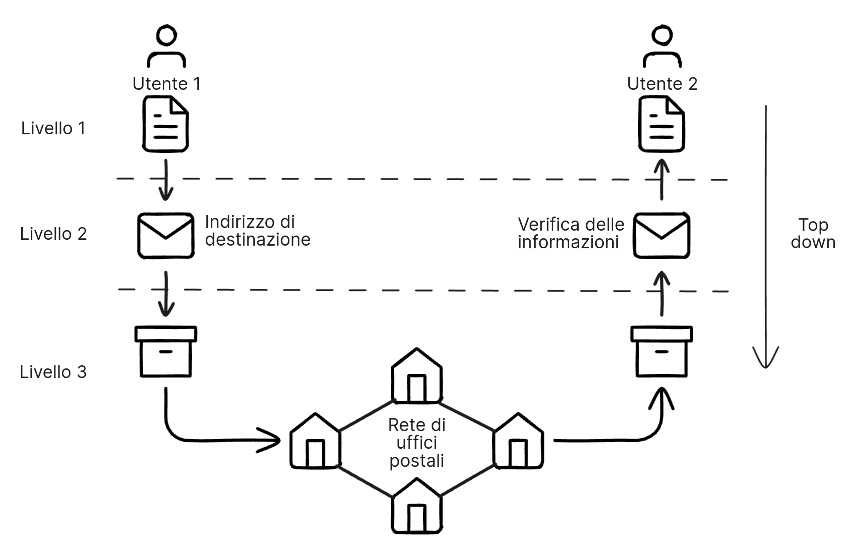
\includegraphics[width=0.95\textwidth]{rete-postale}
      \end{center}
      \caption{Esempio di comunicazione tra 2 utenti}
    \end{figure}

    Il \textbf{Protocollo} è il linguaggio utilizzato per comunicare tra i 2
    utenti, mentre l'\textbf{Architettura di rete} è tutta quella infrastruttura
    che trasporta il messaggio tra i 2 utenti.
  \end{example}
\end{figure}

\noindent
La rappresentazione dei sistemi di comunicazione di solito viene fatta nella modalità
\textbf{top-down}, cioè si parte dal livello applicativo, quello più alto, fino a scendere
nei livelli più bassi in cui si trova la vera e propria architettura della rete.

\section{Architetture di rete}
Di solito si fa riferimento all'architettura più utilizzata, cioè la rete
\textbf{Internet}. Si possono distinguere i seguenti elementi base:
\begin{itemize}
  \item \textbf{Calcolatori (End host)}
  \item \textbf{Router (Intermediate host)}
  \item \textbf{Collegamenti}
\end{itemize}

\subsection{Reti locali}
Le reti locali, o \textbf{LAN} (Local Area Network), sono caratterizzate da un
\textbf{router di bordo} a cui sono collegati gli end host tramite \textbf{cavi fisici}
o collegamenti wireless.
\label{09-10-D1}

\vspace{1em}
\noindent
Per collegare diverse LAN tra loro esiste la \textbf{backbone}, cioè è una rete
di router collegati tra di loro con una topologia
gestita dal gestore della rete. Questi router sono geograficamente distribuiti
su tutto il territorio.
\label{09-10-D2}

\noindent
Nella maggior parte delle volte le connessioni tra i router all'interno della
backbone sono cablate, di solito tramite fibre ottiche, soltanto in rari casi
si usano connessioni wireless.

\subsubsection{Organizzazione del Backbone}
Il backbone è composto da diverse reti che appartengono a diverse organizzazioni
permettendo di creare diverse interconnessioni tra le reti. Queste organizzazioni
si chiamano \textbf{Internet Service Provider} (ISP). Gli ISP hanno diversi livelli:
\begin{enumerate}
  \item \textbf{Livello 1}: Hanno una connessione internazionale
    e quindi sono in grado di comunicare con tutti gli altri ISP.
  \item \textbf{Livello 2}: Lavorano a livello nazionale.
  \item \textbf{Livello 3}: Lavorano a livello locale.
\end{enumerate}

\noindent
Gli ISP di livello 1 sono collegati tra di loro per permettere la comunicazione
tra ISP di livello 1 diversi. Anche gli ISP di livello più basso permettono
la comunicazione tra di loro o tra gli ISP di livello superiore, tutto questo
grazie ad accordi commerciali tra le varie organizzazioni.
\label{09-10-D3}

\noindent
\textbf{Internet} è la \textbf{Rete delle reti}, cioè è la rete che collega
tutti gli ISP tra di loro ed è un organizzazione gerarchica, cioè è sufficiente
creare collegamenti con un sottoinsieme di ISP operanti sul territorio per permettere
il collegamento a tutta la rete.

\noindent
Di conseguenza, per raggiungere un utente, in genere, si segue un percorso gerarchico.
Un esempio è la rete stradale, dove per raggiungere una città si seguono le strade
principali e poi si scende in quelle secondarie.
\label{09-10-D4}

\noindent
La scelta del percorso segue criteri basati su distanza e tempo.

\section{Modalità di comunicazione}
La gestione del trasporto dei messaggi è gestita dalla rete, però con che modalità
trasferisco l'informazione tra 2 utenti?

\subsection{Reti a commutazione di circuito}
È la modalità di commutazione che è stata utilizzata per la prima volta.

\noindent
In questa modalità le risorse (capacità del canale di trasmissione) vengono riservate \textbf{end-to-end}
per la comunicazione, cioè viene letteralmente riservato un circuito che viene
utilizzato dai 2 utenti.
\label{09-10-D5}

\noindent
Ogni canale è completamente dedicato alla comunicazione tra i 2 utenti, quindi
se più utenti vogliono comunicare tra di loro, bisogna riservare altre risorse.

\subsubsection{Vantaggi}
\begin{itemize}
  \item Risorse dedicate
  \item Ritardo deterministico

    \noindent
    \begin{itemize}
      \item \textbf{Ritardo di trasmissione}: Tempo necessario per trasmettere il messaggio
      \item \textbf{Ritardo di propagazione}: Tempo necessario per trasmettere il messaggio
        da un nodo all'altro
    \end{itemize}
    Se il messaggio è grande \( L\,bit \) e il canale riservato è di \( B\,bit/s \),
    allora il tempo di trasmissione sarà:
    \[
    T = \frac{L}{B}
    \] 
    Il ritardo di trasmissione e di propagazione è deterministico, perchè
    dato il circuito di trasmissione, il tempo di trasmissione è noto.
\end{itemize}

\subsubsection{Svantaggi}
Nel corso di utilizzo sporadico si ha uno spreco di risorse, perchè il circuito
viene riservato per tutta la durata della comunicazione, anche se i 2 utenti
non stanno comunicando.
\label{09-10-D6}

\subsection{Reti a commutazione di pacchetto}
È la modalità di commutazione più utilizzata al giorno d'oggi.

\noindent
L'informazione (messaggio) viene suddivisa in \textbf{pacchetti} e ad ogni
pacchetto viene aggiunto un \textbf{header} per permettere:
\begin{itemize}
  \item La consegna del pacchetto stesso
  \item La ricostruzione del messaggio
\end{itemize}

Il messaggio è l'informazione da trasferire, mentre il pacchetto è una porzione
del messaggio stesso.

\noindent
Il messaggio prima della trasmissione viene separato in unità più piccole e a
queste unità viene aggiunta un'intestazione che serve a rendere le unità indipendenti
per poterle trasmettere in modo indipendente. L'intestazione permette la consegna del
pacchetto perchè contiene la destinazione del pacchetto e la ricostruzione del messaggio
perchè contiene il numero di sequenza del pacchetto.
\label{09-10-D7}

\noindent I pacchetti vengono salvati all'interno di un \textbf{buffer}, cioè una
memoria temporanea, in attesa di essere trasmessi. Man mano che i pacchetti
vengono inviati vengono accumulati nel buffer dei router e questo avviene per
qualsiasi collegamento.
\label{09-10-D8}

\noindent
I pacchetti possono arrivare in ordine diverso rispetto a quello di trasmissione,
però grazie all'header è possibile ricostruire il messaggio originale.

\subsubsection{Vantaggi}
\begin{itemize}
  \item Utilizza le risprse solo quando ci sono pacchetti da trasmettere e questo
    viene chiamato
  \item \textbf{Multiplazione statistica}, cioè utilizzo lo stesso
    canale per trasmettere più pacchetti di utenti diversi.
\end{itemize}

\subsubsection{Svantaggi}
\begin{itemize}
  \item Potenziale perdita dei pacchetti: La memoria dei buffer ha una capacità finita,
    quindi se il tasso di ricezione dei pacchetti è superiore al tasso di
    smaltimento del buffer, esso inizia a riempirsi. Le perdite aumentano la
    complessità di gestione della rete.

  \item Ritardi aumentati

    \noindent
    I router prima di trasmettere i pacchetti, deve aspettare di ricevere tutti
    i pacchetti. Questo si chiama \textbf{store \& forward}. Di conseguenza
    più aumentano i router, più aumenta il ritardo di trasmissione.
    \label{09-10-D9}
\end{itemize}

\section{Ritardi di trasmissione}
\label{10-10-D1}
Su un singolo router le componenti principali del ritardo sono:
\begin{itemize}
  \item \textbf{Ritardo di elaborazione al nodo}: Tempo necessario per elaborare
    il pacchetto.
  \item \textbf{Ritardo di accodamento}: È il tempo speso nel buffer prima che
    il pacchetto venga trasmesso ed è la componente principale tra tutti i
    ritardi. (\( \frac{L}{B} \))
  \item \textbf{Ritardo di trasmissione}: Tempo necessario per trasmettere il
    pacchetto.
  \item \textbf{Ritardo di propagazione}: Tempo necessario per trasmettere il
    pacchetto da un nodo all'altro.
\end{itemize}

\subsection{Ordine di grandezza}
Dipende dalla distanza e dalla velocità di trasmissione del collegamento. La
distanza si distingue in:
\begin{itemize}
  \item \textbf{Locale}: \( < 10ms \) 
  \item \textbf{Internazionale}: \( 20-40ms \) 
  \item \textbf{Intercontinentale}: \( > 100ms \)
\end{itemize}

\subsection{Strumenti per calcolare il ritardo end-to-end}
\subsubsection{Ping}
Dati 2 utenti in 2 LAN diverse, il ping manda un pacchetto all'utente di destinazione
e l'utente che lo ha mandato prima o poi riceverà un messaggio di risposta (\textbf{
  echo reply}). Il tempo che passa tra l'invio del pacchetto e la ricezione del
messaggio di risposta è il ritardo end-to-end.

\vspace{1em}
\noindent
Non si può sapere se è asimmetrico o no, cioè se il ritardo di andata è uguale
al ritardo di ritorno, ma si può soltanto calcolare il ritardo totale.
\label{10-10-D2}

\subsubsection{Traceroute}
Vengono mandati 3 messaggi al primo router e si calcolano i tempi di risposta tra
il primo utente e il primo router, poi viene fatta la stessa cosa con i seguenti
router fino ad arrivare all'utente di destinazione.
\label{10-10-D3}

\subsection{Quantità di dati trasferiti}
La quantità di informazioni che si riesce a trasmettere si misura in \( \frac{bit}{s} \)
e questa informazione dipende dalla capacità di tutti i canali di trasmissione
attraversati.

\noindent
Ogni canale avrà una dimensione diversa e si può determinare la banda totale a
disposizione (\textbf{Throughput}) dal \textbf{collo di bottiglia}, cioè dalla minore
capacità di trasmissione tra tutti i canali attraversati.
\label{10-10-D4}


\end{document}
